\documentclass[runningheads]{llncs}

\usepackage{proof}
\usepackage{stmaryrd}
\usepackage{amsmath}
\usepackage{amssymb}
\usepackage{listings}
\usepackage{varwidth}
\usepackage{tikz}
\usepackage{tikz-cd}
\usepackage{nameref}
\usepackage{caption}
\usepackage{subcaption}
% \usepackage{syntax}
% \usepackage{simplebnf}

\usetikzlibrary{backgrounds,fit,decorations.pathreplacing,calc}
\lstset{basicstyle=\ttfamily, mathescape=true, literate={~} {$\sim$}{1}}

\newcommand {\ra} {\rightarrow}
\newcommand {\labinfer} [3] [] {\infer[{\textsc{#1}}]{#2}{#3}}
\newcommand {\Type} {\textsf{Type}}
\newcommand {\Nat} {\textsf{Nat}}
\newcommand {\Bool} {\textsf{Bool}}
\newcommand {\Vect} {\textsf{Vec}}
\newcommand {\ok} {\text{ type}}
\newcommand {\Env} {\textsf{Env}}
\newcommand {\State} {\textsf{State}}
\newcommand {\Value} {\textsf{Value}}
\newcommand {\Locus} {\textsf{Locus}}
\newcommand {\Loc} {\textsf{Location}}
\newcommand {\sem} [1] {\llbracket #1 \rrbracket}
\newcommand {\Esem} [1] {E\sem{#1}}
\newcommand {\Expr} {\textsf{Expr}}
\newcommand {\Cmd} {\textsf{Stmt}}
\newcommand {\CmdTy} {\texttt{Stmt}}
\newcommand {\ExprTy} {\texttt{ExprTy}}
\newcommand {\Apply} {\textsf{Apply}}
\newcommand {\fst} {\ensuremath{\textsf{proj}_1}}
\newcommand {\snd} {\ensuremath{\textsf{proj}_2}}
\newcommand {\Var} {\textsf{Var}}
\newcommand {\Index} {\textsf{Index}}
\newcommand {\Cast} {\textsf{Cast}}
\newcommand {\Rename} {\textsf{Rename}}
\newcommand {\Permute} {\textsf{Permute}}
\newcommand {\loceq} {\approx}

\newcommand{\ket}[1]{\ensuremath{\left|#1\right\rangle}}

\begin{document}

\title{Syntax and Semantics}
\author{}
\institute{}
\maketitle

\section{Testing Framework}

A QSym program can be divided up into two kinds of code:

\begin{enumerate}
  \item Classical parts (these use oracles)
  \item Quantum parts
\end{enumerate}

Information flows between these two kinds of code. The classical parts use \textit{symbolic} execution while the quantum parts are tested using \textit{concrete} execution. Together, these make up a \textit{concolic} testing framework for quantum programs. In Fig~\ref{fig:control-flow}, the classical code uses symbolic execution while the quantum code uses concrete execution.

\begin{figure}
% https://q.uiver.app/#q=WzAsNixbMCwxLCJcXHRleHRub3JtYWx7Q2xhc3NpY2FsIGNvZGV9Il0sWzEsMSwiXFx0ZXh0bm9ybWFse1F1YW50dW0gY29kZX0iXSxbMiwwLCJcXHRleHRub3JtYWx7Q2xhc3NpY2FsIGNvZGV9Il0sWzIsMiwiXFx0ZXh0bm9ybWFse0NsYXNzaWNhbCBjb2RlfSJdLFszLDEsIlxcdGV4dG5vcm1hbHtRdWFudHVtIGNvZGV9Il0sWzQsMSwiXFx0ZXh0bm9ybWFse0NsYXNzaWNhbCBjb2RlfSJdLFsxLDJdLFsxLDNdLFswLDFdLFsyLDRdLFszLDRdLFs0LDVdXQ==
\[\begin{tikzcd}
	&& {\textnormal{Classical code}} \\
	{\textnormal{Classical code}} & {\textnormal{Quantum code}} && {\textnormal{Quantum code}} & {\textnormal{Classical code}} \\
	&& {\textnormal{Classical code}}
	\arrow[from=1-3, to=2-4]
	\arrow[from=2-1, to=2-2]
	\arrow[from=2-2, to=1-3]
	\arrow[from=2-2, to=3-3]
	\arrow[from=2-4, to=2-5]
	\arrow[from=3-3, to=2-4]
\end{tikzcd}\]
  \caption{Control flow of representative program}
  \label{fig:control-flow}
\end{figure}

\section{Syntax}

  \begin{tabular}{lll}
    Locus\; & $\ell$ & ::= $x[i, j)$ $\mid$ $x[i, j) \uplus \ell$\\
    Expression\; & e & ::= $x$ $\mid$ $x[i,j)$ $\mid$ $e + e$ $\mid$ $e \cdot e$\\
    Statement\; & s & ::= s ; s $\mid$ $\Apply$ $\ell$ $e$ $\mid$ $\Cast$ $\ell$ $\ell$
  \end{tabular}

% \begin{center}
% \begin{bnf}
%   s : \Cmd ::= s ; s $\mid$ \Apply\;\ell\;e;;
% \end{bnf}
% \end{center}

\section{Typing Rules}

\[
  \begin{array}{c}
    \fbox{$\Gamma \vdash C : A$}
    \\\\
    \labinfer[T-Apply]{\Gamma \vdash \Apply\;\ell\;e : \CmdTy}
      {\Gamma, \ell \vdash e : \ExprTy}
  \end{array}
\]

\section{Denotational semantics}
A QSym program consists of a list of commands (or ``statements''). These commands can, in turn, involve expressions.


    \fbox{
      \begin{minipage}{\textwidth}
      \[
      \begin{array}{ll}
        \Esem{\cdot} &{}: \Expr \ra \Locus^{+} \ra \State \ra \State\\
                \sem{\cdot} &{}: \Cmd \ra (\State \ra \State)\\
                \Permute &{}: (\Locus \times \Locus) \ra (\Value \ra \Value)\\
                \State &{}= \Loc \ra \Value\\
                \Loc &{}= \Var \times \Index\\
                \ell \loceq \ell
          \end{array}
        \]
      \end{minipage}
}

\subsection{Semantics of expressions}

Expressions are, in general, \textit{open} expressions: they generally have free variables. These expressions will consist of typical bitwise operations and arithmetic operations. The free variables refer to locations in quantum state.

\[
  \begin{array}{c}
    % \Esem{e_1, e_2}(a, b) = \Esem{e_2}(b) \circ \Esem{e_1}(a)\\\\
    \Esem{\ell}(b, \ell)\phi = \phi[\ell \mapsto b]
    % \Esem{e_1 + e_2}a = 
  \end{array}
\]

\subsection{Semantics of statements}

A statement performs some transformation to the quantum state. This will typically involve evaluating some given expression.

\subsubsection{``Apply'' semantics}

The expression $e$ in the command $\ell \Apply e$ will generally by an \textit{open} expression. That is, it typically has free variables. The value of this variable ranges over the quantum states. This is a kind of ``map'' operation over the (probability-weighted) possibilities. This amounts to applying the expression to the value part of the matching entry in the $\State$. The value part is the second item of an entry (the first item is the locus).

An entry will ``match'' the apply expression if the locus of the entry is the same as the locus of the apply, up to permutation.

\subsubsection{``Permute'' semantics}

The $\Permute(\ell, \ell')$ command will take two ``equivalent'' loci (see the previous subsection). That is, a pair of loci which are the same up to permutation. Then, it will permute the bits of the value at that locus in such a way that the loci will match exactly.

For example, if we have $\Permute(x[0, 3) \uplus y[0, 2))(y[0, 2)\uplus x[0, 3))$ then we would swap the two identified bit vectors in the quantum state.

\subsubsection{Step-by-Step Example}

Consider the following program, which puts its input into an evenly weighted superposition (a Bell pair) and inverts the bits in one of the elements of the array:

\begin{lstlisting}[frame=single]
  q[0] <- H;

  if (q[0]) {
    q[1] <- (x => x + 1);
  }
\end{lstlisting}

We will build the circuit by going through this program line-by-line. We start with a circuit that just consists of input wires. This is the circuit before the main part of the program (at this point, we've only taken into account the free variables).\\

\begin{minipage}{.5\textwidth}
\begin{lstlisting}[frame=single]
  q[0] <- H;

  if (q[0]) {
    q[1] <- (x => x + 1);
  }
\end{lstlisting}
\end{minipage}%
~~~
\begin{minipage}{.5\textwidth}
% Based on https://tex.stackexchange.com/a/44270/186240
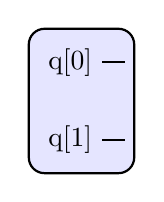
\begin{tikzpicture}[thick]
    % `operator' will only be used by Hadamard (H) gates here.
    % `phase' is used for controlled phase gates (dots).
    % `surround' is used for the background box.
    \tikzstyle{operator} = [draw,fill=white,minimum size=1.5em] 
    \tikzstyle{phase} = [draw,fill,shape=circle,minimum size=5pt,inner sep=0pt]
    \tikzstyle{surround} = [fill=blue!10,thick,draw=black,rounded corners=2mm]
    %
    \matrix[row sep=0.4cm, column sep=0.8cm] (circuit) {
      \node (q0) {q[0]}; &[-0.5cm] 
    \coordinate (end0); \\

      \node (q1) {q[1]}; &[-0.5cm] 
    \coordinate (end1); \\
    %
  };
  \begin{pgfonlayer}{background}
        % Draw background box.
    \node[surround] (background) [fit = (q0) (end0) (q1) (end1) ] {};
        % Draw lines.
        \draw[thick] (q0) -- (end0)  (q1) -- (end1);
    \end{pgfonlayer}
\end{tikzpicture}
\end{minipage}

Next, we deal with the apply with the Hadamard gate.\\

\begin{minipage}{.5\textwidth}
\begin{lstlisting}[frame=single, escapechar=!] 
  !\colorbox{yellow}{q[0] <- H;}!

  if (q[0]) {
    q[1] <- (x => x + 1);
  }
\end{lstlisting}
  \end{minipage}%
  ~~~
\begin{minipage}{.5\textwidth}
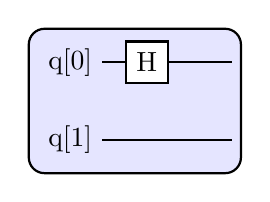
\begin{tikzpicture}[thick]
    % `operator' will only be used by Hadamard (H) gates here.
    % `phase' is used for controlled phase gates (dots).
    % `surround' is used for the background box.
    \tikzstyle{operator} = [draw,fill=white,minimum size=1.5em] 
    \tikzstyle{phase} = [draw,fill,shape=circle,minimum size=5pt,inner sep=0pt]
    \tikzstyle{surround} = [fill=blue!10,thick,draw=black,rounded corners=2mm]
    %
    \matrix[row sep=0.4cm, column sep=0.8cm] (circuit) {
      \node (q0) {q[0]}; &[-0.5cm] 
      \node[operator] (H21) {H}; &
    \coordinate (end0); \\

      \node (q1) {q[1]}; &[-0.5cm] 
    &[-0.3cm]
    \coordinate (end1); \\
    %
  };
  \begin{pgfonlayer}{background}
        % Draw background box.
    \node[surround] (background) [fit = (q0) (end0) (q1) (end1) ] {};
        % Draw lines.
        \draw[thick] (q0) -- (end0)  (q1) -- (end1);
    \end{pgfonlayer}
\end{tikzpicture}
  \end{minipage}

Now, the \texttt{if} condition.\\

\begin{minipage}{.5\textwidth}
\begin{lstlisting}[frame=single, escapechar=!] 
  q[0] <- H;

  !\colorbox{yellow}{if (q[0]) \{}!
    q[1] <- (x => x + 1);
  }
\end{lstlisting}
\end{minipage}%
~~~
\begin{minipage}{.5\textwidth}
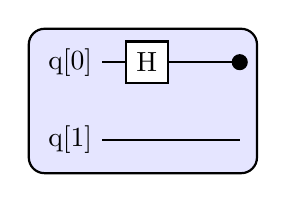
\begin{tikzpicture}[thick]
    % `operator' will only be used by Hadamard (H) gates here.
    % `phase' is used for controlled phase gates (dots).
    % `surround' is used for the background box.
    \tikzstyle{operator} = [draw,fill=white,minimum size=1.5em] 
    \tikzstyle{phase} = [draw,fill,shape=circle,minimum size=5pt,inner sep=0pt]
    \tikzstyle{surround} = [fill=blue!10,thick,draw=black,rounded corners=2mm]
    \tikzstyle{circlewc} = [draw,circle,cross,minimum width=0.3 cm]
    %
    \matrix[row sep=0.4cm, column sep=0.8cm] (circuit) {
      \node (q0) {q[0]}; &[-0.5cm] 
      \node[operator] (H21) {H}; &
      \node[phase] (P12) {};
    \coordinate (end0); \\

      \node (q1) {q[1]}; &[-0.5cm] 
    &[-0.3cm]
    \coordinate (end1); \\
    %
  };
  \begin{pgfonlayer}{background}
        % Draw background box.
    \node[surround] (background) [fit = (q0) (end0) (q1) (end1) (P12) ] {};
        % Draw lines.
        \draw[thick] (q0) -- (end0)  (q1) -- (end1);
    \end{pgfonlayer}
\end{tikzpicture}
\end{minipage}

Finally, the body of the \texttt{if}.\\

\begin{minipage}{.5\textwidth}
\begin{lstlisting}[frame=single, escapechar=!] 
  q[0] <- H;

  if (q[0]) {
    !\colorbox{yellow}{q[1] <- (x => x + 1);}!
  }
\end{lstlisting}
\end{minipage}%
~~~
\begin{minipage}{.5\textwidth}
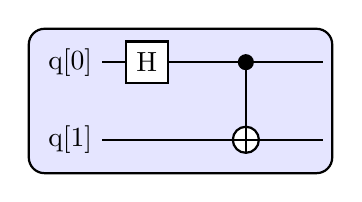
\begin{tikzpicture}[thick]
    % `operator' will only be used by Hadamard (H) gates here.
    % `phase' is used for controlled phase gates (dots).
    % `surround' is used for the background box.
    \tikzstyle{operator} = [draw,fill=white,minimum size=1.5em] 
    \tikzstyle{phase} = [draw,fill,shape=circle,minimum size=5pt,inner sep=0pt]
    \tikzstyle{surround} = [fill=blue!10,thick,draw=black,rounded corners=2mm]

    \tikzstyle{cross} =[path picture={ 
\draw[thick,black](path picture bounding box.north) -- (path picture bounding box.south) (path picture bounding box.west) -- (path picture bounding box.east);
}],
    \tikzstyle{circlewc} = [draw,fill=white,circle,cross,minimum width=0.3 cm]
    %
    \matrix[row sep=0.4cm, column sep=0.8cm] (circuit) {
      \node (q0) {q[0]}; &[-0.5cm] 
      \node[operator] (H21) {H}; &
      \node[phase] (P12) {}; &
    \coordinate (end0); \\

      \node (q1) {q[1]}; &[-0.5cm]  &
      \node[circlewc] (H21) {}; &
    \coordinate (end1); \\
    %
  };
  \begin{pgfonlayer}{background}
        % Draw background box.
    \node[surround] (background) [fit = (q0) (end0) (q1) (end1) ] {};
        % Draw lines.
        \draw[thick] (q0) -- (end0)  (q1) -- (end1)  (P12) -- (H21);
    \end{pgfonlayer}
\end{tikzpicture}
\end{minipage}

\subsubsection{Loop example}

Here, we look at the GHZ example with $n=4$.

\begin{minipage}{.5\textwidth}
  \begin{lstlisting}[frame=single]
  x[0] <- H;
  for j in [1, 4) && x[j-1]
    x[j] <- x[j] + 1;
  \end{lstlisting}
\end{minipage}
~~~
\begin{minipage}{.5\textwidth}
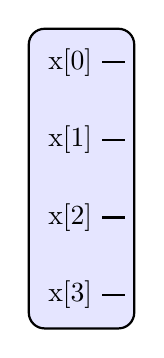
\begin{tikzpicture}[thick]
    % `operator' will only be used by Hadamard (H) gates here.
    % `phase' is used for controlled phase gates (dots).
    % `surround' is used for the background box.
    \tikzstyle{operator} = [draw,fill=white,minimum size=1.5em] 
    \tikzstyle{phase} = [draw,fill,shape=circle,minimum size=5pt,inner sep=0pt]
    \tikzstyle{surround} = [fill=blue!10,thick,draw=black,rounded corners=2mm]
    \tikzstyle{cross} =[path picture={ 
\draw[thick,black](path picture bounding box.north) -- (path picture bounding box.south) (path picture bounding box.west) -- (path picture bounding box.east);
}],
    \tikzstyle{circlewc} = [draw,fill=white,circle,cross,minimum width=0.3 cm]
    %
    \matrix[row sep=0.4cm, column sep=0.8cm] (circuit) {
      \node (q0) {x[0]}; &[-0.5cm] 
    \coordinate (end0); \\

      \node (q1) {x[1]}; &[-0.5cm] 
    \coordinate (end1); \\

      \node (q2) {x[2]}; &[-0.5cm] 
    \coordinate (end2); \\

      \node (q3) {x[3]}; &[-0.5cm] 
    \coordinate (end3); \\
    %
  };
  \begin{pgfonlayer}{background}
        % Draw background box.
    \node[surround] (background) [fit = (q0) (end0) (q1) (end1) (q2) (end2) (q3) (end3) ] {};
        % Draw lines.
        \draw[thick] (q0) -- (end0)  (q1) -- (end1)
                     (q2) -- (end2)  (q3) -- (end3);
    \end{pgfonlayer}
\end{tikzpicture}
\end{minipage}

Step 1.\\

\begin{minipage}{.5\textwidth}
  \begin{lstlisting}[frame=single, escapechar=!]
  !\colorbox{yellow}{x[0] <- H;}!
  for j in [1, 4) && x[j-1]
    x[j] <- x[j] + 1;
  \end{lstlisting}
\end{minipage}
~~~
\begin{minipage}{.5\textwidth}
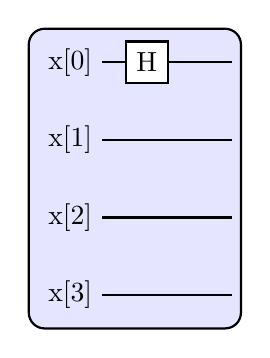
\begin{tikzpicture}[thick]
    % `operator' will only be used by Hadamard (H) gates here.
    % `phase' is used for controlled phase gates (dots).
    % `surround' is used for the background box.
    \tikzstyle{operator} = [draw,fill=white,minimum size=1.5em] 
    \tikzstyle{phase} = [draw,fill,shape=circle,minimum size=5pt,inner sep=0pt]
    \tikzstyle{surround} = [fill=blue!10,thick,draw=black,rounded corners=2mm]
    \tikzstyle{cross} =[path picture={ 
\draw[thick,black](path picture bounding box.north) -- (path picture bounding box.south) (path picture bounding box.west) -- (path picture bounding box.east);
}],
    \tikzstyle{circlewc} = [draw,fill=white,circle,cross,minimum width=0.3 cm]
    %
    \matrix[row sep=0.4cm, column sep=0.8cm] (circuit) {
      \node (q0) {x[0]}; &[-0.5cm]
      \node[operator] (H21) {H}; &
    \coordinate (end0); \\

      \node (q1) {x[1]}; &[-0.5cm] &
    \coordinate (end1); \\

      \node (q2) {x[2]}; &[-0.5cm] &
    \coordinate (end2); \\

      \node (q3) {x[3]}; &[-0.5cm] &
    \coordinate (end3); \\
    %
  };
  \begin{pgfonlayer}{background}
        % Draw background box.
    \node[surround] (background) [fit = (q0) (end0) (q1) (end1) (q2) (end2) (q3) (end3) ] {};
        % Draw lines.
        \draw[thick] (q0) -- (H21)  (H21) -- (end0)  (q1) -- (end1)
                     (q2) -- (end2)  (q3) -- (end3);
    \end{pgfonlayer}
\end{tikzpicture}
\end{minipage}

Step 2.\\

\begin{minipage}{.5\textwidth}
  \begin{lstlisting}[frame=single, escapechar=!]
  x[0] <- H;
  !\colorbox{yellow}{for j in [1, 4) \&\& x[j-1]}!
    x[j] <- x[j] + 1;
  \end{lstlisting}
\end{minipage}
~~~
\begin{minipage}{.5\textwidth}
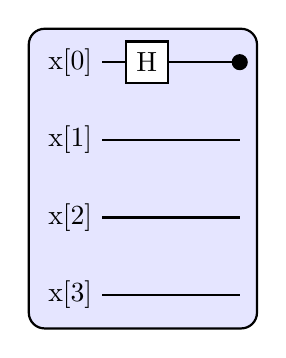
\begin{tikzpicture}[thick]
    % `operator' will only be used by Hadamard (H) gates here.
    % `phase' is used for controlled phase gates (dots).
    % `surround' is used for the background box.
    \tikzstyle{operator} = [draw,fill=white,minimum size=1.5em] 
    \tikzstyle{phase} = [draw,fill,shape=circle,minimum size=5pt,inner sep=0pt]
    \tikzstyle{surround} = [fill=blue!10,thick,draw=black,rounded corners=2mm]
    \tikzstyle{cross} =[path picture={ 
\draw[thick,black](path picture bounding box.north) -- (path picture bounding box.south) (path picture bounding box.west) -- (path picture bounding box.east);
}],
    \tikzstyle{circlewc} = [draw,fill=white,circle,cross,minimum width=0.3 cm]
    %
    \matrix[row sep=0.4cm, column sep=0.8cm] (circuit) {
      \node (q0) {x[0]}; &[-0.5cm]
      \node[operator] (H21) {H}; &
      \node[phase] (P12) {};
    \coordinate (end0); \\

      \node (q1) {x[1]}; &[-0.5cm] &
    \coordinate (end1); \\

      \node (q2) {x[2]}; &[-0.5cm] &
    \coordinate (end2); \\

      \node (q3) {x[3]}; &[-0.5cm] &
    \coordinate (end3); \\
    %
  };
  \begin{pgfonlayer}{background}
        % Draw background box.
    \node[surround] (background) [fit = (q0) (end0) (q1) (end1) (q2) (end2) (q3) (end3) (P12) ] {};
        % Draw lines.
        \draw[thick] (q0) -- (H21)  (H21) -- (end0)  (q1) -- (end1)
                     (q2) -- (end2)  (q3) -- (end3);
    \end{pgfonlayer}
\end{tikzpicture}
\end{minipage}

Step 3.\\

\begin{minipage}{.5\textwidth}
  \begin{lstlisting}[frame=single, escapechar=!]
  x[0] <- H;
  for j in [1, 4) && x[j-1]
    !\colorbox{yellow}{x[j] <- x[j] + 1;}!
  \end{lstlisting}
\end{minipage}
~~~
\begin{minipage}{.5\textwidth}
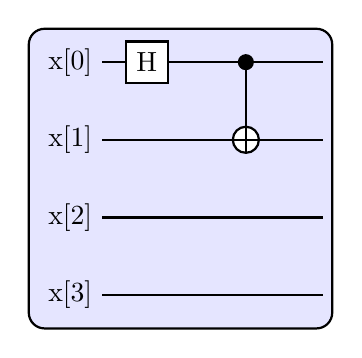
\begin{tikzpicture}[thick]
    % `operator' will only be used by Hadamard (H) gates here.
    % `phase' is used for controlled phase gates (dots).
    % `surround' is used for the background box.
    \tikzstyle{operator} = [draw,fill=white,minimum size=1.5em] 
    \tikzstyle{phase} = [draw,fill,shape=circle,minimum size=5pt,inner sep=0pt]
    \tikzstyle{surround} = [fill=blue!10,thick,draw=black,rounded corners=2mm]
    \tikzstyle{cross} =[path picture={ 
\draw[thick,black](path picture bounding box.north) -- (path picture bounding box.south) (path picture bounding box.west) -- (path picture bounding box.east);
}],
    \tikzstyle{circlewc} = [draw,fill=white,circle,cross,minimum width=0.3 cm]
    %
    \matrix[row sep=0.4cm, column sep=0.8cm] (circuit) {
      \node (q0) {x[0]}; &[-0.5cm]
      \node[operator] (H21) {H}; &
      \node[phase] (P12) {}; &
    \coordinate (end0); \\

      \node (q1) {x[1]}; &[-0.5cm] &
      \node[circlewc] (C1) {}; &
    \coordinate (end1); \\

      \node (q2) {x[2]}; &[-0.5cm] & &
    \coordinate (end2); \\

      \node (q3) {x[3]}; &[-0.5cm] & &
    \coordinate (end3); \\
    %
  };
  \begin{pgfonlayer}{background}
        % Draw background box.
    \node[surround] (background) [fit = (q0) (end0) (q1) (end1) (q2) (end2) (q3) (end3) (P12) ] {};
        % Draw lines.
        \draw[thick] (q0) -- (H21)  (H21) -- (end0)  (q1) -- (end1)
                     (q2) -- (end2)  (q3) -- (end3)
                     (P12) -- (C1);
    \end{pgfonlayer}
\end{tikzpicture}
\end{minipage}

Step 4.\\

\begin{minipage}{.5\textwidth}
  \begin{lstlisting}[frame=single, escapechar=!]
  x[0] <- H;
  !\colorbox{yellow}{for j in [1, 4) \&\& x[j-1]}!
    x[j] <- x[j] + 1;
  \end{lstlisting}
\end{minipage}
~~~
\begin{minipage}{.5\textwidth}
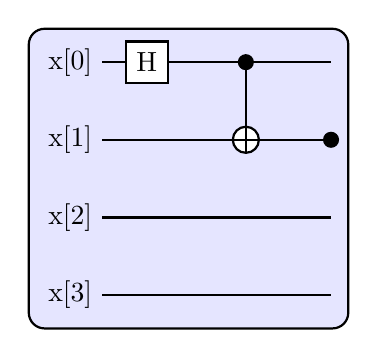
\begin{tikzpicture}[thick]
    % `operator' will only be used by Hadamard (H) gates here.
    % `phase' is used for controlled phase gates (dots).
    % `surround' is used for the background box.
    \tikzstyle{operator} = [draw,fill=white,minimum size=1.5em] 
    \tikzstyle{phase} = [draw,fill,shape=circle,minimum size=5pt,inner sep=0pt]
    \tikzstyle{surround} = [fill=blue!10,thick,draw=black,rounded corners=2mm]
    \tikzstyle{cross} =[path picture={ 
\draw[thick,black](path picture bounding box.north) -- (path picture bounding box.south) (path picture bounding box.west) -- (path picture bounding box.east);
}],
    \tikzstyle{circlewc} = [draw,fill=white,circle,cross,minimum width=0.3 cm]
    %
    \matrix[row sep=0.4cm, column sep=0.8cm] (circuit) {
      \node (q0) {x[0]}; &[-0.5cm]
      \node[operator] (H21) {H}; &
      \node[phase] (P12) {}; &
    \coordinate (end0); \\

      \node (q1) {x[1]}; &[-0.5cm] &
      \node[circlewc] (C1) {}; &
      \node[phase] (P13) {};
    \coordinate (end1); \\

      \node (q2) {x[2]}; &[-0.5cm] & &
    \coordinate (end2); \\

      \node (q3) {x[3]}; &[-0.5cm] & &
    \coordinate (end3); \\
    %
  };
  \begin{pgfonlayer}{background}
        % Draw background box.
    \node[surround] (background) [fit = (q0) (end0) (q1) (end1) (q2) (end2) (q3) (end3) (P12) (P13) ] {};
        % Draw lines.
        \draw[thick] (q0) -- (H21)  (H21) -- (end0)  (q1) -- (end1)
                     (q2) -- (end2)  (q3) -- (end3)
                     (P12) -- (C1);
    \end{pgfonlayer}
\end{tikzpicture}
\end{minipage}

Step 5.\\

\begin{minipage}{.5\textwidth}
  \begin{lstlisting}[frame=single, escapechar=!]
  x[0] <- H;
  for j in [1, 4) && x[j-1]
    !\colorbox{yellow}{x[j] <- x[j] + 1;}!
  \end{lstlisting}
\end{minipage}
~~~
\begin{minipage}{.5\textwidth}
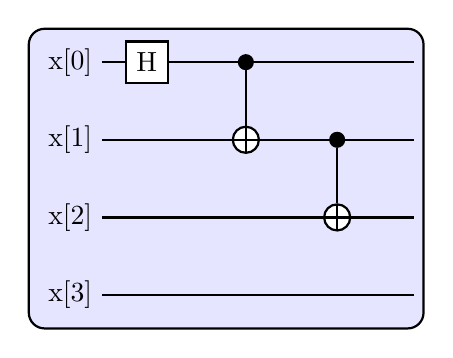
\begin{tikzpicture}[thick]
    % `operator' will only be used by Hadamard (H) gates here.
    % `phase' is used for controlled phase gates (dots).
    % `surround' is used for the background box.
    \tikzstyle{operator} = [draw,fill=white,minimum size=1.5em] 
    \tikzstyle{phase} = [draw,fill,shape=circle,minimum size=5pt,inner sep=0pt]
    \tikzstyle{surround} = [fill=blue!10,thick,draw=black,rounded corners=2mm]
    \tikzstyle{cross} =[path picture={ 
\draw[thick,black](path picture bounding box.north) -- (path picture bounding box.south) (path picture bounding box.west) -- (path picture bounding box.east);
}],
    \tikzstyle{circlewc} = [draw,fill=white,circle,cross,minimum width=0.3 cm]
    %
    \matrix[row sep=0.4cm, column sep=0.8cm] (circuit) {
      \node (q0) {x[0]}; &[-0.5cm]
      \node[operator] (H21) {H}; &
      \node[phase] (P12) {}; & &
    \coordinate (end0); \\

      \node (q1) {x[1]}; &[-0.5cm] &
      \node[circlewc] (C1) {}; &
      \node[phase] (P13) {}; &
    \coordinate (end1); \\

      \node (q2) {x[2]}; &[-0.5cm] & &
      \node[circlewc] (C2) {}; &
    \coordinate (end2); \\

      \node (q3) {x[3]}; &[-0.5cm] & & &
    \coordinate (end3); \\
    %
  };
  \begin{pgfonlayer}{background}
        % Draw background box.
    \node[surround] (background) [fit = (q0) (end0) (q1) (end1) (q2) (end2) (q3) (end3) (P12) (P13) ] {};
        % Draw lines.
        \draw[thick] (q0) -- (H21)  (H21) -- (end0)  (q1) -- (end1)
                     (q2) -- (end2)  (q3) -- (end3)
                     (P12) -- (C1)  (P13) -- (C2);
    \end{pgfonlayer}
\end{tikzpicture}
\end{minipage}

Step 6.\\

\begin{minipage}{.5\textwidth}
  \begin{lstlisting}[frame=single, escapechar=!]
  x[0] <- H;
  !\colorbox{yellow}{for j in [1, 4) \&\& x[j-1]}!
    x[j] <- x[j] + 1;
  \end{lstlisting}
\end{minipage}
~~~
\begin{minipage}{.5\textwidth}
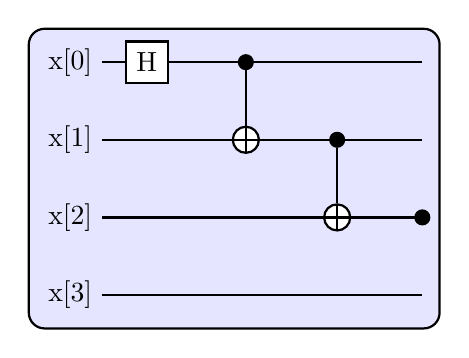
\begin{tikzpicture}[thick]
    % `operator' will only be used by Hadamard (H) gates here.
    % `phase' is used for controlled phase gates (dots).
    % `surround' is used for the background box.
    \tikzstyle{operator} = [draw,fill=white,minimum size=1.5em] 
    \tikzstyle{phase} = [draw,fill,shape=circle,minimum size=5pt,inner sep=0pt]
    \tikzstyle{surround} = [fill=blue!10,thick,draw=black,rounded corners=2mm]
    \tikzstyle{cross} =[path picture={ 
\draw[thick,black](path picture bounding box.north) -- (path picture bounding box.south) (path picture bounding box.west) -- (path picture bounding box.east);
}],
    \tikzstyle{circlewc} = [draw,fill=white,circle,cross,minimum width=0.3 cm]
    %
    \matrix[row sep=0.4cm, column sep=0.8cm] (circuit) {
      \node (q0) {x[0]}; &[-0.5cm]
      \node[operator] (H21) {H}; &
      \node[phase] (P12) {}; & &
    \coordinate (end0); \\

      \node (q1) {x[1]}; &[-0.5cm] &
      \node[circlewc] (C1) {}; &
      \node[phase] (P13) {}; &
    \coordinate (end1); \\

      \node (q2) {x[2]}; &[-0.5cm] & &
      \node[circlewc] (C2) {}; &
      \node[phase] (P14) {};
    \coordinate (end2); \\

      \node (q3) {x[3]}; &[-0.5cm] & & &
    \coordinate (end3); \\
    %
  };
  \begin{pgfonlayer}{background}
        % Draw background box.
    \node[surround] (background) [fit = (q0) (end0) (q1) (end1) (q2) (end2) (q3) (end3) (P12) (P13) (P14) ] {};
        % Draw lines.
        \draw[thick] (q0) -- (H21)  (H21) -- (end0)  (q1) -- (end1)
                     (q2) -- (end2)  (q3) -- (end3)
                     (P12) -- (C1)  (P13) -- (C2);
    \end{pgfonlayer}
\end{tikzpicture}
\end{minipage}

Step 7.\\

\begin{minipage}{.5\textwidth}
  \begin{lstlisting}[frame=single, escapechar=!]
  x[0] <- H;
  for j in [1, 4) && x[j-1]
    !\colorbox{yellow}{x[j] <- x[j] + 1;}!
  \end{lstlisting}
\end{minipage}
~~~
\begin{minipage}{.5\textwidth}
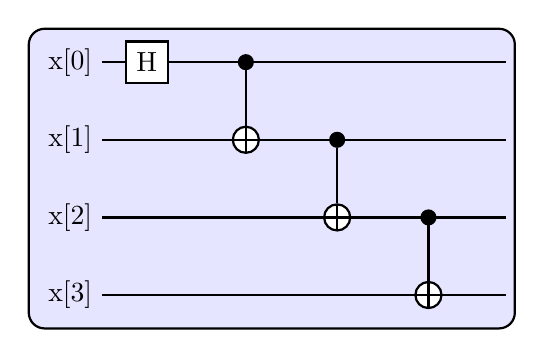
\begin{tikzpicture}[thick]
    % `operator' will only be used by Hadamard (H) gates here.
    % `phase' is used for controlled phase gates (dots).
    % `surround' is used for the background box.
    \tikzstyle{operator} = [draw,fill=white,minimum size=1.5em] 
    \tikzstyle{phase} = [draw,fill,shape=circle,minimum size=5pt,inner sep=0pt]
    \tikzstyle{surround} = [fill=blue!10,thick,draw=black,rounded corners=2mm]
    \tikzstyle{cross} =[path picture={ 
\draw[thick,black](path picture bounding box.north) -- (path picture bounding box.south) (path picture bounding box.west) -- (path picture bounding box.east);
}],
    \tikzstyle{circlewc} = [draw,fill=white,circle,cross,minimum width=0.3 cm]
    %
    \matrix[row sep=0.4cm, column sep=0.8cm] (circuit) {
      \node (q0) {x[0]}; &[-0.5cm]
      \node[operator] (H21) {H}; &
      \node[phase] (P12) {}; & & &
    \coordinate (end0); \\

      \node (q1) {x[1]}; &[-0.5cm] &
      \node[circlewc] (C1) {}; &
      \node[phase] (P13) {}; & &
    \coordinate (end1); \\

      \node (q2) {x[2]}; &[-0.5cm] & &
      \node[circlewc] (C2) {}; &
      \node[phase] (P14) {}; &
    \coordinate (end2); \\

      \node (q3) {x[3]}; &[-0.5cm] & & &
      \node[circlewc] (C3) {}; &
    \coordinate (end3); \\
    %
  };
  \begin{pgfonlayer}{background}
        % Draw background box.
    \node[surround] (background) [fit = (q0) (end0) (q1) (end1) (q2) (end2) (q3) (end3) (P12) (P13) (P14) ] {};
        % Draw lines.
        \draw[thick] (q0) -- (H21)  (H21) -- (end0)  (q1) -- (end1)
                     (q2) -- (end2)  (q3) -- (end3)
                     (P12) -- (C1)  (P13) -- (C2)  (P14) -- (C3);
    \end{pgfonlayer}
\end{tikzpicture}
\end{minipage}



\subsubsection{Denotation}

\[
  \begin{array}{c}
    \sem{\Apply\;\ell\;e}\phi = \phi[(\ell, b) \mapsto
               (\ell, \Esem{e}(b, \ell)\phi)]\\\\
    \sem{\Cast\;\ell\;\ell'}\phi = \phi[(\ell', a) \mapsto (\ell, \Permute(\ell, \ell')(a))]\\\\
    \sem{c;c'} = \sem{c'} \circ \sem{c}
  \end{array}
\]

\textbf{TODO}: But what about the permutations?

\end{document}
